% Software Roboter (C++)
% Zuständig: Leander

\section{Software - Roboter}
\label{sec:software_robots}
Für die Programmierung der Mikrocontroller verwenden wir PlatformIO.
%
PlatformIO ist eine Alternative zur Arduino-IDE,
welche mithilfe von Plugins in viele IDEs wie z.B. VSCode und CLion integriert werden kann.
%
Alternativ kann man PlatformIO auch über die Kommandozeile bedienen.
%
Vorteile von PlatformIO gegenüber der Arduino-IDE sind u.A. schnelleres Kompilieren,
ordentliche Auto-Vervollständigung,
statische Code-Analyse (Linting),
und ein schön geregeltes System für Bibliotheken.
%
Was die Ansteuerung der einzelnen Roboter angeht, folgen wir so gut wie möglich dem DRY-Prinzip (``Don't repeat yourself''),
um Redundanzen zu vermeiden und dadurch den Wartungsaufwand möglichst gering zu halten.

\subsection{Kameras}
\label{subsec:robots_cams}
Wir verwenden jeweils ein ESP32-CAM AI-Thinker Modul zur erweiterten
Fernüberwachung der Roboter.
%
Dieses verbindet sich über WLAN mit dem \texttt{IoT}-Netzwerk und bietet über HTTP einen MJPEG-Videostream an.
%
Die drei Videostreams (einer pro Roboter) werden dann im Web-Interface
zusätzlich zu den LiDAR-Umgebungsdaten angezeigt,
um das räumliche Vorstellungsvermögen der Benutzer zu unterstützen.
%
Die Videodaten werden also nicht automatisch verarbeitet und zur autonomen Steuerung verwendet,
sondern dienen nur als weiterer Input für die Bediener.
\begin{figure}[H]
    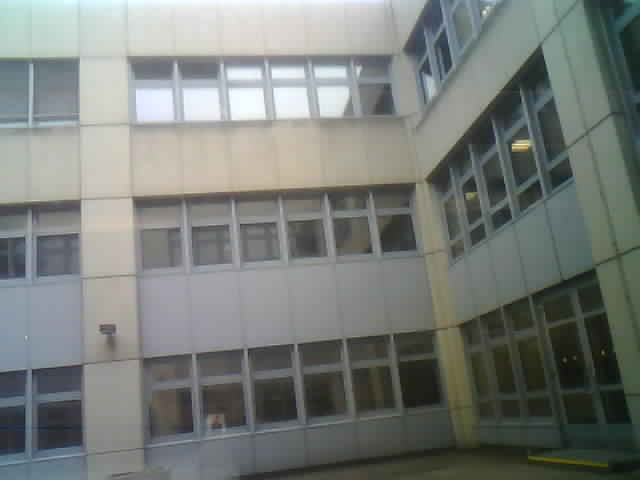
\includegraphics[width=0.7\textwidth, center]{img/cam_erstes_bild.png}
    \caption{Erstes empfangenes Bild der ESP32-CAM}
    \label{fig:cam_erstes_bild}
\end{figure}

\subsection{Core-Bibliothek}
\label{subec:robots_core}
Die Core-Bibliothek bildet eine weiter Abstrahierungsschicht zu den Funktionalitäten der Roboter-Hardware.
%
In unserem Modell stellt die Arduino-Bibliothek die erste Abstrahierungsschicht dar,
während die Code-Bibliothek diese weiter vereinfacht.
%
Durch diese Abstrahierung werden die Programme für die einzelnen Roboter um ein Vielfaches vereinfacht und dementsprechend übersichtlicher.
%
Wir können also die hier definierte Logik für jeden Roboter wiederverwenden,
anstatt drei mal fast genau das Gleiche zu programmieren.
%
Die Core-Bibliothek übernimmt alles von der WLAN-Verbindung,
über die Fernsteuerung per WebSockets,
bis hin zum Umschalten der einzelnen Pins zur Ansteuerung der Motortreiber.
%
Die Programmierung der einzelnen Roboter beschränkt sich also darauf,
die einzelnen Komponenten zu konfigurieren und miteinander zu verbinden.
%
Da Herr Gastgeber während der Projektwoche 2023/24 (Siehe Abschnitt \ref{sec:vorgeschichte}) bereits viel Zeit darin investiert hat,
die Bibliothek so modular und wiederverwendbar wie möglich zu gestalten,
konnten wir diese mit nur wenigen Modifikationen für unsere Diplomarbeit nutzen,
obwohl wir einen ganz anderen Hardwareaufbau verwenden.

\subsection{Guide}
\label{subsec:software_guide}

\subsection{Tamerlan}
\label{subsec:software_tamerlan}

\subsection{Bambi}
\label{subsec:software_bambi}